\section{Modeling edit distance} \label{sec:apdx:model_distance}
In this section, we describe the details for the three models we used to analyze the edit distance data.

\subsection{Model 1: Edit Distance per Option} \label{sec:apdx:model_distance_option}

\subsubsection{Dependent variables}
The dependent variable for this model is the edit total distance accumulated for an option $D_i$. Distance is a positive continuous variable.

\subsubsection{Independent variables}
The independent variables for this model are the length of the option $L_i$, modeled as a ordinal variable (Equation~\ref{eq:distance_model_1_eta_ordinal}); interface type $I_i$, modeled as a categorical variable; user effect $U_i$ as categorical variables. The ordinal variable $L_i$ consists of a intercept $\mu_L$ and added effect $\beta_L$, given the interface ordinal value. Since we only have two interfaces, we do not have to worry about the interval between two or more interfaces. Priors are weakly informed in Equation~\ref{eq:priors_global_mean}. We reparamtereized $U_i$ given the sparser sample from each participant. This is written in Equations~\ref{eq:distance_model_1_user_effect}. Both reparameterization contains an intercept and scaling of the effect due to this user. This will imporve sampling efficiency and help the model converge. Relavent priors are written in Equations~\ref{eq:priors_global_mean} and~\ref{eq:priors_sigma_U}. We added an interaction effect between length and interface type $\phi_{ij}$ described in Equation~\ref{eq:distance_model_1_lkj}. Similiar to cognitive load model, the interaction effect used a non-centered parameterization constrained by an LKJ prior to account for correlations. Priors for the interaction effect is listed in Equations~\ref{eq:priors_sigma_phi} and~\ref{eq:priors_L_Omega}. Detailed description can be found in Appendix~\ref{apdx:model_tlx}.

\subsubsection{Overall model and Likelihood function}
We modeled the dependent variable using an Exponential distribution (Equation~\ref{eq:distance_model_1}). Since Exponential distribution takes in a positive value, we transformed it as Equation~\ref{eq:transformation_model_1}. The observed outcome variable $D_i$ represents the response for the $i$-th observation parameterized by the latent predictor $\eta_i$. $\eta_i$ is described in Equation~\ref{eq:distance_model_1_eta} as the regression with length, interface, the interaction effect and the interface.

\begin{align}
    D_i \sim \text{Exponential}(\lambda_i) \label{eq:distance_model_1} \\
    \lambda_i = \exp(\eta_i) \label{eq:transformation_model_1}\\
    \eta_i = \gamma_i + \beta_I[I_i] + \phi_{ij} + U_i \label{eq:distance_model_1_eta} \\
    \gamma_i = \mu_L + \beta_L \cdot L_i \label{eq:distance_model_1_eta_ordinal} \\
    \phi_{ij} = L_{\Omega} \cdot (\sigma_{\phi} \odot z_{\phi}) \label{eq:distance_model_1_lkj} \\
    U_i = \mu_U + \sigma_U \cdot z_U \label{eq:distance_model_1_user_effect}
\end{align}

Priors are defined as:
\begin{align}
    \mu_L, \mu_I, \mu_U, \beta_L, \beta_I, z_{\phi}, z_U &\sim \mathcal{N}(0, 1) \label{eq:priors_global_mean} \\
    \sigma_{\phi} \sim \text{HalfNormal}(0.5) \label{eq:priors_sigma_phi} \\
    \sigma_U \sim \text{Exponential}(0.5) \label{eq:priors_sigma_U} \\
    L_{\Omega} \sim \text{LKJ}(3) \label{eq:priors_L_Omega}
\end{align}

\subsection{Model 2: Edit Distance with Separate Mean and Variance Predictors} \label{sec:apdx:model_distance_variance}

\subsubsection{Dependent Variables}
The dependent variable for this model is the edit distance (with directions) $D_i$, a positive edit distance refers to participants moving downward. A negtaitve edit distrance refers to a upward movement.

\subsubsection{Overall Model}
We modeled the dependent variable $D_i$ using a Normal distribution (Equation~\ref{eq:distance_model_2_likelihood}). Since the goal of this model, unlike some, aims to model the variance since we believe participants in two-phase interface would exhibit less oscillation then the text interface. Hence, we model independent variables effecting both $\mu$ and $\sigma$ independently for this analysis to exaime this hypothesis.

\subsubsection{Independent Variables}
The independent variables for this model are:
\begin{itemize}
    \item \textbf{Length of the option $L_i$}: Modeled as an ordinal variable. Since we will be modeling both $\mu_i$ and $\sigma$ of a Normal distribution, Equation~\ref{eq:distance_model_2_gamma_mu} and ~\ref{eq:distance_model_2_gamma_sigma} reflects the ordinal variable. Both formula consists of a intercept $\mu_{L,\mu}, \mu_{L,\sigma}$ and added effect $\beta_{L,\mu}, \beta_{L,\sigma}$, given the interface ordinal value. Since we only have two interfaces, we do not have to worry about the interval between two or more interfaces. Priors of both ordinal relationship are weakly informed in Equation~\ref{eq:priors_distance_model_2_mean} and~\ref{eq:priors_distance_model_2_variance}
    \item \textbf{Interface type $I_i$}: Modeled as a categorical variable. Following the previous discussion, they are drawn from a hyperprior. We reparamtereized this independent variable given the added complexity of this model. This is written in Equations~\ref{eq:distance_model_2_beta_I_mu} and~\ref{eq:distance_model_2_beta_I_sigma}. Both reparameterization contains an intercept and scaling of the effect due to this interface. Relavent priors are written in Equations~\ref{eq:priors_distance_model_2_mean},~\ref{eq:priors_distance_model_2_variance}, and~\ref{eq:priors_interface_distance_model_2}.
    \item \textbf{User effect $U_i$}: Users are modeled as categorical variables. Following the interface, it is also reparamtereized as Equations~\ref{eq:distance_model_2_user_mu} and~\ref{eq:distance_model_2_user_sigma}. Priors are defined in Equations~\ref{eq:priors_distance_model_2_mean},~\ref{eq:priors_distance_model_2_variance}, and~\ref{eq:priors_sigma_U_distance_model_2}
    \item \textbf{Interaction between length and interface type $\phi_{ij}$}: Similiar to the interaction effect for cognitive load, we used a non-centered parameterization constrained by an LKJ prior to account for correlations. This is described by Equation~\ref{eq:distance_model_2_phi_mu} and~\ref{eq:distance_model_2_phi_sigma}. Refer to Appendix~\ref{apdx:model_tlx} for a more detailed explaination. Relevent priors are described in Equation~\ref{eq:priors_L_Omega_distance_model_2} and~\ref{eq:priors_sigma_phi_distance_model_2}. We relaxed the LKJ priors comapred to the cognitive load model given the complexity of the model allowing a lesser belief in correlation among the two variables.
\end{itemize}

\subsubsection{Likelihood Function}
Given these independent variables, we model both $\mu$ and $\sigma$ as linear regressions. While we can directly model $mu$ (Equation~\ref{eq:distance_model_2_mu}), we need to make sure $sigma$ is strictly positive, we applied a transformation described in~\ref{eq:distance_model_2_sigma}. Hence, both $\mu_i$ and $\log(\sigma_{\text{obs},i})$ now regresses on the linear combination of length, interface, interaction effect, and user effect. 

\begin{align}
    D_i &\sim \text{Normal}(\mu_i, \sigma_{\text{obs},i}) \label{eq:distance_model_2_likelihood} \\
    \mu_i &= \gamma_{\mu,i} + \beta_{I,\mu}[I_i] + \phi_{\mu,ij} + U_{\mu,i} \label{eq:distance_model_2_mu} \\
    \gamma_{\mu,i} &= \mu_{L,\mu} + \beta_{L,\mu} \cdot L_i \label{eq:distance_model_2_gamma_mu} \\
    \beta_{I,\mu}[I_i] &= \mu_{I,\mu} + \sigma_{I,\mu} \cdot \text{I}_{\mu,I_i} \label{eq:distance_model_2_beta_I_mu} \\
    \phi_{\mu,ij} &= L_{\Omega,\mu} \cdot (\sigma_{\phi,\mu} \odot z_{\phi,\mu}) \label{eq:distance_model_2_phi_mu} \\
    U_{\mu,i} &= \mu_{U,\mu} + \sigma_{U,\mu} \cdot z_{U,\mu,i} \label{eq:distance_model_2_user_mu} \\
    \log(\sigma_{\text{obs},i}) &= \gamma_{\sigma,i} + \beta_{I,\sigma}[I_i] + \phi_{\sigma,ij} + U_{\sigma,i} \label{eq:distance_model_2_sigma} \\
    \gamma_{\sigma,i} &= \mu_{L,\sigma} + \beta_{L,\sigma} \cdot L_i \label{eq:distance_model_2_gamma_sigma} \\
    \beta_{I,\sigma}[I_i] &= \mu_{I,\sigma} + \sigma_{I,\sigma} \cdot \text{I}_{\sigma,I_i} \label{eq:distance_model_2_beta_I_sigma} \\
    \phi_{\sigma,ij} &= L_{\Omega,\sigma} \cdot (\sigma_{\phi,\sigma} \odot z_{\phi,\sigma}) \label{eq:distance_model_2_phi_sigma} \\
    U_{\sigma,i} &= \mu_{U,\sigma} + \sigma_{U,\sigma} \cdot z_{U,\sigma,i} \label{eq:distance_model_2_user_sigma}
\end{align}

\subsubsection{Priors}
Priors are defined as:
\begin{align}
    \mu_{L,\mu}, \mu_{I,\mu}, \mu_{U,\mu}, \beta_{L,\mu}, \beta_{I,\mu}, z_{\phi,\mu}, z_{U,\mu,i} &\sim \mathcal{N}(0, 1) \label{eq:priors_distance_model_2_mean} \\
    \mu_{L,\sigma}, \mu_{I,\sigma}, \mu_{U,\sigma}, \beta_{L,\sigma}, \beta_{I,\sigma}, z_{\phi,\sigma}, z_{U,\sigma,i} &\sim \mathcal{N}(0, 1) \label{eq:priors_distance_model_2_variance} \\
    \sigma_{I,\mu}, \sigma_{I,\sigma} &\sim  \text{HalfNormal}(0.5) \label{eq:priors_interface_distance_model_2} \\
    \sigma_{\phi,\mu}, \sigma_{\phi,\sigma} &\sim \text{HalfNormal}(0.5) \label{eq:priors_sigma_phi_distance_model_2} \\
    \sigma_{U,\mu}, \sigma_{U,\sigma} &\sim \text{Exponential}(0.5) \label{eq:priors_sigma_U_distance_model_2} \\
    L_{\Omega,\mu}, L_{\Omega,\sigma} &\sim \text{LKJ}(3) \label{eq:priors_L_Omega_distance_model_2}
\end{align}

\subsubsection{Model Results}
Here we provide all pairwise comparisons for the variance which the main text only provided the comparison within the same survey length. Figure~\ref{fig:bayesian_distance_variance} shows the pairwise comparison of the variance of edit distance in the first row followed by the effect size in the second row. An notable result that we omit from the main text is that if we compare the variance between the long and short text, and the variance between the long and short two-phase, we see that the text group had three times the standard deviation compared to the two-phase group. This indicates that the organization phase minimize the added length of the survey.

\begin{figure}[h!]
    \centering
    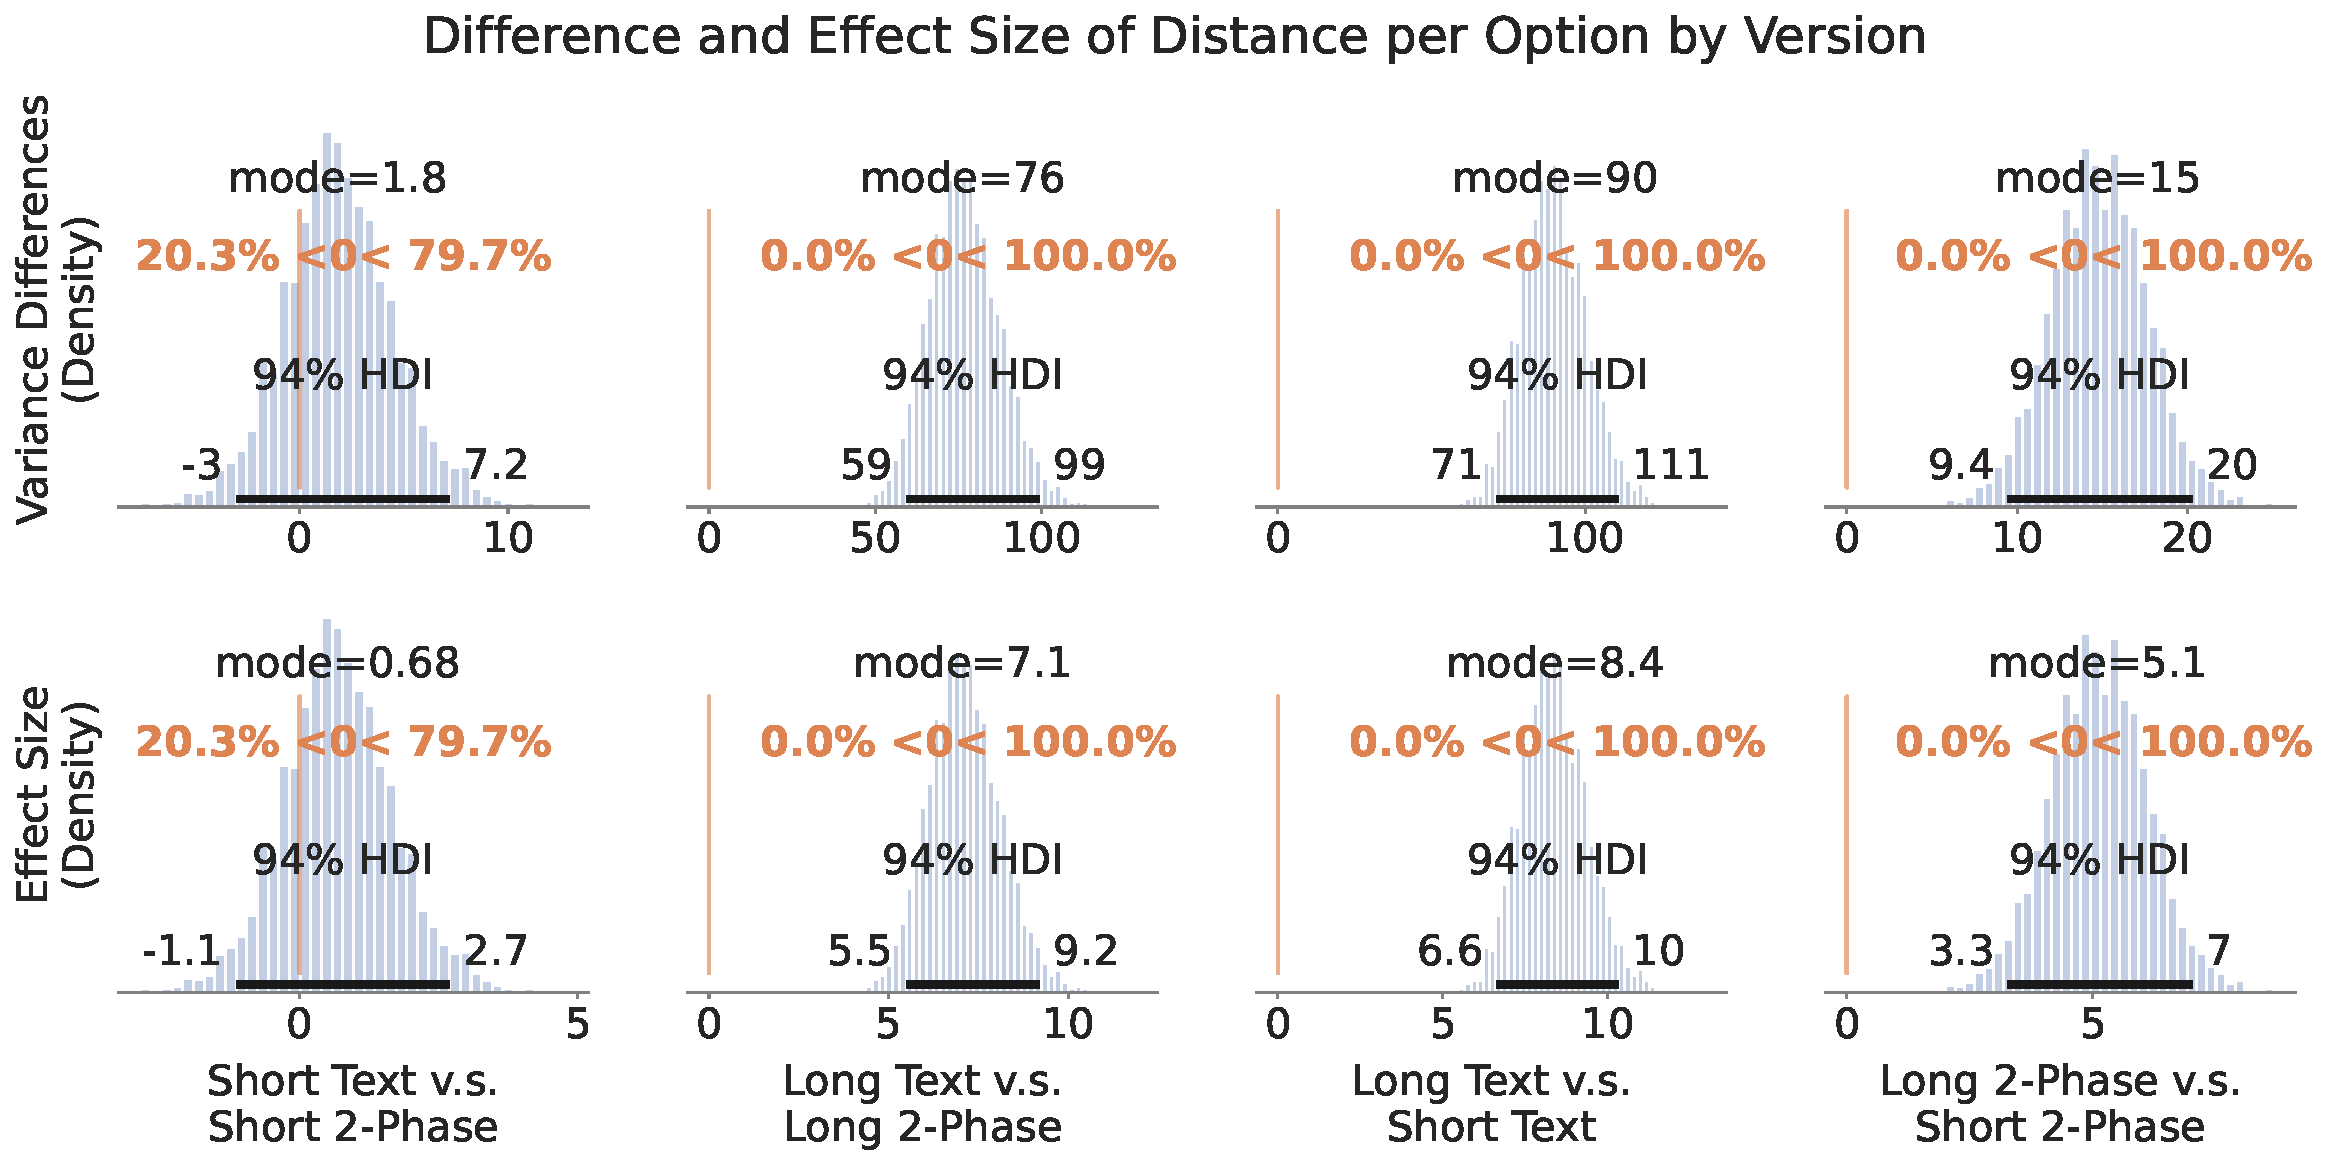
\includegraphics[width=\textwidth]{content/image/distance/distance_diff_per_option_effect_size_by_version_all.pdf}
    \caption{Differences in the variance of edit distance by version.}
    \label{fig:bayesian_distance_variance}
\end{figure}

\newpage
\subsection{Model 3: Cumulative Edit Distance for long QS} \label{sec:apdx:model_cum_distance}

\subsubsection{Dependent Variables}
The dependent variable for this model is the cumulative edit distance \( D_i \). Cumulative edit distance is a positive continuous variable measured at each step within a version for each user.

\subsubsection{Independent Variables}
The independent variables for this model involve the following. Steps refers to the $n$-th step when completing QS ($S_i$), and interface version refers to the type of interface used ($V_i$). User-specific effects are included as ($U_i$). Both interface versions and user-specific effects are modeled with their own hyperpriors to capture variability across these groups. 

Equation~\ref{eq:model3_prior_beta}, refers to interface versions, $\beta_v[V_i]$ are drawn from a Normal distribution with hyperparameters defined in Equations~\ref{eq:model3_prior_beta_mu} and~\ref{eq:model3_prior_beta_sigma} corresponding to the mean and variance of this distribution. 

Instead of directly sampling $U_i$ from a hyper distribution, we reparameterize it to account for limited data for each user. This reparameterization is presented in Equation~\ref{eq:model3_user_mu}. $\mu_{U}$ models the overall mean user effect from users, with $\sigma_{U}$ used to capture variability in user effects (Equation~\ref{eq:model3_prior_user}). A standard normal random variable, Equation~\ref{eq:model3_prior_z} introduced individual randomness for each user.


\subsubsection{Overall Model and Likelihood Function}
We modeled the dependent variable $D_i$ using a Truncated Normal distribution (Equation~\ref{eq:model3_likelihood}). The observation-specific standard deviation, drawn from a Half-Normal distribution as described in Equation~\ref{eq:model3_prior_sigma}. The latent predictors $\mu_i$ is modeled as a regression equation (Equation~\ref{eq:model3_mu}). This equation reflects our intuition that the effects from versions and user differences are amplified by steps as the participants complete the survey. The intercept $\alpha_{\text{shared}}$ is assigned a prior described in Equation~\ref{eq:model3_prior_shared}. The effect of users $\sigma_{U}$ and version $\beta_v[V_i]$ are amplified by the step number $S_i$.


\begin{align}
    D_i &\sim \text{TruncatedNormal}(\mu_i, \sigma_{\text{obs},i}, \text{lower}=0) \label{eq:model3_likelihood} \\
    \mu_i &= \alpha_{\text{shared}} + \beta_v[V_i] \cdot S_i + U_i \cdot S_i \label{eq:model3_mu} \\
    U_i &= \mu_{U} + \sigma_{U} \cdot z_{U,i} \label{eq:model3_user_mu}
\end{align}

Priors used in this model are listed.
\begin{align}
    \sigma_{\text{obs},i} &\sim \text{HalfNormal}(0.3) \label{eq:model3_prior_sigma} \\
    \alpha_{\text{shared}} &\sim \mathcal{N}(2.0, 0.5) \label{eq:model3_prior_shared} \\
    \mu_{U}, \sigma_{U} &\sim \mathcal{N}(0, 1), \text{ HalfNormal}(0.1) \label{eq:model3_prior_user} \\
    z_{U,i} &\sim \mathcal{N}(0, 1) \label{eq:model3_prior_z} \\
    \beta_v[V_i] &\sim \mathcal{N}(\mu_{\beta}, \sigma_{\beta}) \label{eq:model3_prior_beta} \\
    \mu_{\beta} &\sim \mathcal{N}(0.05, 0.05) \label{eq:model3_prior_beta_mu}\\
    \sigma_{\beta} &\sim \text{HalfNormal}(0.1) \label{eq:model3_prior_beta_sigma}
\end{align}
